
\documentclass{article}
\usepackage[utf8]{inputenc}
\usepackage[spanish]{babel}
\usepackage{graphicx}
\usepackage{geometry}
\usepackage{enumerate}
\usepackage{titlesec}
\usepackage{float}
\usepackage{listings}
\usepackage{xcolor}
\usepackage{amsmath}

\geometry{letterpaper, margin = 1.5cm}


\newcommand{\codefontsize}{\fontsize{12}{12}}
\lstset{
	language=C,
	basicstyle=\codefontsize\ttfamily\color{white},
	keywordstyle=\color{blue},
	commentstyle=\color{green},
	stringstyle=\color{red},
	numbers=left,
	numberstyle=\tiny\color{black},
	stepnumber=1,
	numbersep=10pt,
	backgroundcolor=\color{blue!20!black},
	showspaces=false,
	showstringspaces=false,
	showtabs=false,
	tabsize=4,
	captionpos=b,
	breaklines=true,
	breakatwhitespace=true,
	escapeinside={(*@}{@*)},
	frame=single
}

%Datos de la Portada
\title{Introducción a la Programación \\ Practica 4}
\author{Medina Martinez Jonathan Jason \\ 2023640061}
\date{25 de marzo del 2023}

\begin{document} %Inicio del Documento

\fontsize{12}{16}\selectfont

\begin{figure}[t] %Logos Portada


\includegraphics[width=2.5 cm]{Logo1.jpeg}
\hfill

\includegraphics[width=3 cm]{Logo2.png}

\end{figure}

\maketitle %Titulo Portada
\newpage

\tableofcontents %Indice
\newpage

\section{Objetivo}

Desarrollar programas aplicando el método de la burbuja y resolver problemas con arreglos bidimensionales.

\section{Introducción}

Esta practica muestra los códigos y la solución de la práctica 3 de Introducción a la Programación, que consiste en el desarrollo de programas utilizando el método de la burbuja y la manipulación de arreglos bidimensionales.

\newpage

\section{Desarrollo}

Realice los siguientes programas en C.

\subsection{Burbuja}

Cree un programa que solicite al usuario un numero de muestras \textit{n} y genere un arreglo de números pseudoaleatorios dimensión \textit{n}.
Los dígitos deberán estar en el rango de \textit{50} a \textit{300}. Una vez generado el arreglo, ordenarlo de mayor a menor utilizando el método de la burbuja.
\par
El programa deberá mostrar ambos arreglos, el generado y ordenado.

\subsubsection{Código 1}

\begin{lstlisting}
/**
* @file programa1.c
* @author Medina Martinez Jonathan Jason (jmedinam1702@alumno.ipn.mx)
* @brief 
* @version 0.1
* @date 2023-03-23
* 
* @copyrigth GPlv3
* 
*/

#include <stdio.h>
#include <stdlib.h>
#include <time.h>

void generar_arreglo_aleatorio(int arr[], int n);
void ordenar_arreglo(int arr[], int n);
void imprimir_arreglo(int arr[], int n);
void imprimir_texto(char text[]);

int main()
{
	int n = 0;
	
	char text1[] = "Ingrese el valor de n";
	imprimir_texto(text1);
	scanf("%d",&n);
	
	int arr[n];
	generar_arreglo_aleatorio(arr, n);
	
	char text2[] = "Arreglo ordenado de mayor a menor:";
	imprimir_texto(text2);
	imprimir_arreglo(arr, n);
	
	ordenar_arreglo(arr, n);
	char text3[] = "Arreglo generado:";
	imprimir_texto(text3);
	
	imprimir_arreglo(arr, n);
	
	return 0;
}

/// @brief Genera un arreglo aleatorio de una dimension dado
/// @param arr El arreglo generada
/// @param n La dimension del arreglo
void generar_arreglo_aleatorio(int arr[], int n) {
	srand(time(NULL));
	for (int i = 0; i < n; i++)
	{
		arr[i] = (rand() % 500) + 1;
	}
}

/// @brief Ordena un arreglo de mayor a menor
/// @param arr El arreglo a ordenar
/// @param n La dimension del arreglo
void ordenar_arreglo(int arr[], int n) {
	int aux = 0, i = 0, j = 0;
	for (i = 0; i < n; i++)
	{
		for (j = 0; j < n - 1 -i; j++)
		{
			if (arr[j] > arr[j + 1])
			{
				aux = arr[j];
				arr[j] = arr[j + 1];
				arr[j + 1] = aux;
			}
		}
	}
}

/// @brief Imprime un arreglo
/// @param arr El arreglo a imprimir
/// @param n La dimension del arreglo
void imprimir_arreglo(int arr[], int n) {
	for (int i = 0; i < n; i++) {
		printf("%d ", arr[i]);
	}
	printf("\n\n");
}

/// @brief Imprime un texto
/// @param text el texto a imprimir
void imprimir_texto(char text[]) {
	printf("\n\n%s\n\n", text);
}
\end{lstlisting}

\subsubsection{Ejecución}

\begin{figure}[H]
	\centering
	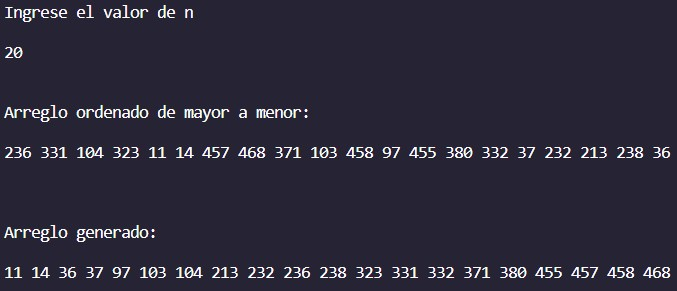
\includegraphics[width = 15cm]{img1.jpg}
\end{figure}
\newpage

\subsection{Calculadora de Matrices}

Cree un programa que

\begin{enumerate}
	\item Defina una matriz \textit{A} de tamaño \textit{3 × 3}.
	\item Defina una matriz \textit{B} de tamaño \textit{3 × 3}.
	\item Solicite al usuario los elementos de la matriz \textit{A} y \textit{B}.
	\item Calcule la suma de \textit{A} mas \textit{B} y muestre en pantalla el resultado.
	\item Calcule la resta de \textit{A} menos \textit{B} y muestre en pantalla el resultado.
	\item Calcule la multiplicación de \textit{A} por \textit{B} y muestre en pantalla el resultado.
\end{enumerate}

\subsubsection{Código 2}

\begin{lstlisting}
/**
* @file programa2.c
* @author Medina Martinez Jonathan Jason (jmedinam1702@alumno.ipn.mx)
* @brief 
* @version 0.1
* @date 2023-03-24
* 
* @copyrigth GPlv3
* 
*/

#include <stdio.h>

void pedir_elementos(int matriz[3][3]);
void suma_matrices(int matrizA[3][3], int matrizB[3][3], int matrizC[3][3]);
void resta_matrices(int matrizA[3][3], int matrizB[3][3], int matrizC[3][3]);
void multiplicacion_matrices(int matrizA[3][3], int matrizB[3][3], int matrizC[3][3]);
void imprimir_matriz(int matrizC[3][3]);
void imprimir_texto(char text[]);

int main() {
	int A[3][3], B[3][3], C[3][3];

	char text1[] = "Ingrese los elementos de la matriz A:";
	imprimir_texto(text1);
	pedir_elementos(A);

	char text2[] = "Ingrese los elementos de la matriz B:";
	imprimir_texto(text2);
	pedir_elementos(B);

	char text3[] = "La suma de A + B es:";
	imprimir_texto(text3);
	suma_matrices(A, B, C);
	imprimir_matriz(C);

	char text4[] = "La resta de A - B es:";
	imprimir_texto(text4);
	resta_matrices(A, B, C);
	imprimir_matriz(C);

	char text5[] = "La multiplicacion de A x B es:";
	imprimir_texto(text5);
	multiplicacion_matrices(A, B, C);
	imprimir_matriz(C);
	
	return 0;
}

/// @brief Pide los elementos de la matriz
/// @param matriz La matriz en la que se guardan los elementos
void pedir_elementos(int matriz[3][3]) {
	for (int i = 0; i < 3; i++) {
		for (int j = 0; j < 3; j++) {
			scanf("%d", &matriz[i][j]);
		}
	}
}

/// @brief Suma 2 matrices
/// @param matrizA Una de las matrices a sumar
/// @param matrizB Una de las matrices a sumar
/// @param matrizC La matriz resultante de la suma
void suma_matrices(int matrizA[3][3], int matrizB[3][3], int matrizC[3][3]) {
	for (int i = 0; i < 3; i++) {
		for (int j = 0; j < 3; j++) {
			matrizC[i][j] = matrizA[i][j] + matrizB[i][j];
		}
	}
}

/// @brief Resta 2 matrices
/// @param matrizA Una de las matrices a restar
/// @param matrizB Una de las matrices a restar
/// @param matrizC La matriz resultante de la resta
void resta_matrices(int matrizA[3][3], int matrizB[3][3], int matrizC[3][3]) {
	for (int i = 0; i < 3; i++) {
		for (int j = 0; j < 3; j++) {
			matrizC[i][j] = matrizA[i][j] - matrizB[i][j];
		}
	}
}

/// @brief Multiplica 2 matrices
/// @param matrizA Una de las matrices a multiplicar
/// @param matrizB Una de las matrices a multiplicar
/// @param matrizC La matriz resultante de la multiplicacion
void multiplicacion_matrices(int matrizA[3][3], int matrizB[3][3], int matrizC[3][3]) {
	for (int i = 0; i < 3; i++) {
		for (int j = 0; j < 3; j++) {
			matrizC[i][j] = 0;
			for (int k = 0; k < 3; k++) {
				matrizC[i][j] += matrizA[i][k] * matrizB[k][j];
			}
		}
	}
}

/// @brief Imprime una matriz
/// @param matriz C 
void imprimir_matriz(int matrizC[3][3]) {
	for (int i = 0; i < 3; i++) {
		for (int j = 0; j < 3; j++) {
			printf("%4d ", matrizC[i][j]);
		}
		printf("\n");
	}
	printf("\n");
}

/// @brief Imprime un texto
/// @param text el texto a imprimir
void imprimir_texto(char text[]) {
		printf("\n\n%s\n\n", text);
}
\end{lstlisting}

\subsubsection{Ejecución}

\begin{figure}[H]
	\centering
	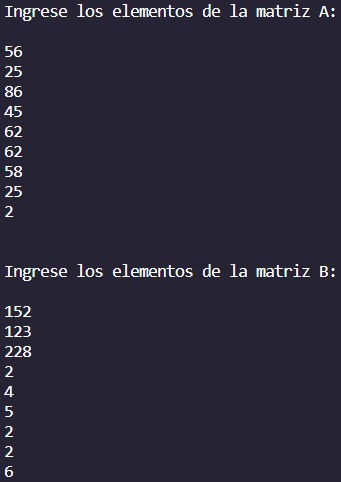
\includegraphics[height = 12cm]{img2a.jpg}
	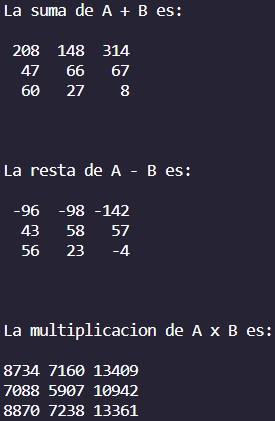
\includegraphics[height = 12cm]{img2b.jpg}
\end{figure}

\subsection{Sistema de Ecuaciones}

\begin{enumerate}
	\item Tomando como base la definición anterior, cree un programa que permita resolver el siguiente sistema de ecuaciones:
	\begin{align*}
		2x - 4y - 3z &= 15 \\
		x + 5y - 5z &= 5 \\
		4x + 2y + 67z &= 20
	\end{align*}
\subsubsection{Código 3}
\begin{lstlisting}
/**
* @file programa3.c
* @author Medina Martinez Jonathan Jason (jmedinam1702@alumno.ipn.mx)
* @brief 
* @version 0.1
* @date 2023-03-24
* 
* @copyrigth GPlv3
* 
*/
	
#include <stdio.h>
	
int main() {
		
	float A[3][3] = {{2, -4, -3}, {1, 5, -5}, {4, 2, 67}};
	float B[3] = {15, 5, 20};
		
	float invA[3][3];
	float detA = A[0][0] * (A[1][1] * A[2][2] - A[2][1] * A[1][2])
	- A[0][1] * (A[1][0] * A[2][2] - A[2][0] * A[1][2])
	+ A[0][2] * (A[1][0] * A[2][1] - A[2][0] * A[1][1]);
		
	invA[0][0] = (A[1][1] * A[2][2] - A[2][1] * A[1][2]) / detA;
	invA[0][1] = (A[0][2] * A[2][1] - A[2][2] * A[0][1]) / detA;
	invA[0][2] = (A[0][1] * A[1][2] - A[1][1] * A[0][2]) / detA;
		
	invA[1][0] = (A[1][2] * A[2][0] - A[2][2] * A[1][0]) / detA;
	invA[1][1] = (A[0][0] * A[2][2] - A[2][0] * A[0][2]) / detA;
	invA[1][2] = (A[0][2] * A[1][0] - A[1][2] * A[0][0]) / detA;
		
	invA[2][0] = (A[1][0] * A[2][1] - A[2][0] * A[1][1]) / detA;
	invA[2][1] = (A[0][1] * A[2][0] - A[2][1] * A[0][0]) / detA;
	invA[2][2] = (A[0][0] * A[1][1] - A[1][0] * A[0][1]) / detA;
		
	float X[3];
	X[0] = invA[0][0] * B[0] + invA[0][1] *
	B[1] + invA[0][2] * B[2];
	X[1] = invA[1][0] * B[0] + invA[1][1] *
	B[1] + invA[1][2] * B[2];
	X[2] = invA[2][0] * B[0] + invA[2][1] *
	B[1] + invA[2][2] * B[2];
		
	printf("La solucion es: \n");
	printf("x = %f \n", X[0]);
	printf("y = %f \n", X[1]);
	printf("z = %f \n", X[2]);
		
	return 0;
}
\end{lstlisting}
\item Compruebe los resultados obtenidos haciendo el producto punto de cada fila de A con el vector columna X.
\begin{figure}[H]
	\centering
	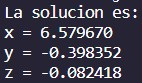
\includegraphics[height = 2cm]{img3a.jpg}
\end{figure}

\item Modifique su programa para que permita resolver cualquier sistema de tres ecuaciones.
\subsubsection{Código 3 Modificado}
\begin{lstlisting}
/**
* @file programa3.c
* @author Medina Martinez Jonathan Jason (jmedinam1702@alumno.ipn.mx)
* @brief 
* @version 0.1
* @date 2023-03-24
* 
* @copyrigth GPlv3
* 
*/

#include <stdio.h>

int main() {
	float A[3][3];
	float B[3];
	
	printf("Calculadora de sistemas de ecuaciones lineales 3x3\n\n");
	printf("Ejemplo de sistema de ecuaciones lineales 3x3:\n");
	printf("A[0][0]x + A[0][1]y + A[0][2]z = B[1]\n");
	printf("A[1][0]x + A[1][1]y + A[1][2]z = B[2]\n");
	printf("A[2][0]x + A[2][1]y + A[2][2]z = B[3]\n\n");
	
	printf("Ingrese los elementos de la matriz A: \n");
	for(int i=0; i<3; i++) {
		for(int j=0; j<3; j++) {
			printf("A[%d][%d] = ", i, j);
			scanf("%f", &A[i][j]);
		}
	}
	
	printf("Ingrese los elementos del vector B: \n");
	for(int i=0; i<3; i++) {
		printf("B[%d] = ", i);
		scanf("%f", &B[i]);
	}
	
	float invA[3][3];
	float detA = A[0][0] * (A[1][1] * A[2][2] - A[2][1] * A[1][2])
	- A[0][1] * (A[1][0] * A[2][2] - A[2][0] * A[1][2])
	+ A[0][2] * (A[1][0] * A[2][1] - A[2][0] * A[1][1]);
	
	invA[0][0] = (A[1][1] * A[2][2] - A[2][1] * A[1][2]) / detA;
	invA[0][1] = (A[0][2] * A[2][1] - A[2][2] * A[0][1]) / detA;
	invA[0][2] = (A[0][1] * A[1][2] - A[1][1] * A[0][2]) / detA;
	
	invA[1][0] = (A[1][2] * A[2][0] - A[2][2] * A[1][0]) / detA;
	invA[1][1] = (A[0][0] * A[2][2] - A[2][0] * A[0][2]) / detA;
	invA[1][2] = (A[0][2] * A[1][0] - A[1][2] * A[0][0]) / detA;
	
	invA[2][0] = (A[1][0] * A[2][1] - A[2][0] * A[1][1]) / detA;
	invA[2][1] = (A[0][1] * A[2][0] - A[2][1] * A[0][0]) / detA;
	invA[2][2] = (A[0][0] * A[1][1] - A[1][0] * A[0][1]) / detA;
	
	float X[3];
	X[0] = invA[0][0] * B[0] + invA[0][1] * B[1] + invA[0][2] * B[2];
	X[1] = invA[1][0] * B[0] + invA[1][1] * B[1] + invA[1][2] * B[2];
	X[2] = invA[2][0] * B[0] + invA[2][1] * B[1] + invA[2][2] * B[2];
	
	printf("La solucion es: \n");
	printf("x = %f \n", X[0]);
	printf("y = %f \n", X[1]);
	printf("z = %f \n", X[2]);
	
	return 0;
}
\end{lstlisting}

\subsubsection{Ejecución}

\begin{figure}[H]
	\centering
	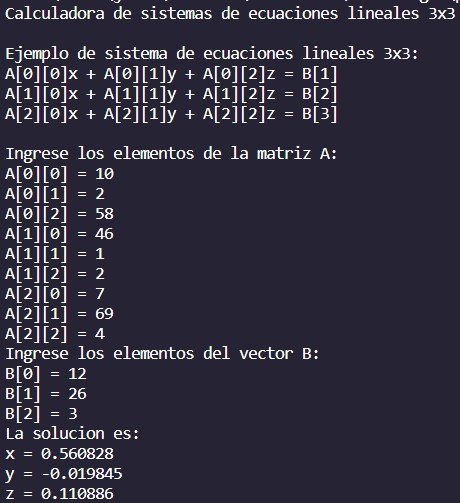
\includegraphics[width = 8cm]{img3b.jpg}
\end{figure}

\end{enumerate}

\newpage

\section{Conclusión}

La práctica 3 de Introducción a la Programación ha permitido desarrollar habilidades en la manipulación de arreglos y el uso del método de la burbuja para ordenarlos. Los programas creados en C han sido efectivos en la generación y ordenamiento de los arreglos, y demuestran la aplicación de los conceptos teóricos aprendidos en clase.

\end{document}